\begin{apendicesenv}

\partapendices

\chapter{Análise das Missões Anteriores}
\label{apendicea}

Analisou-se algumas missões CubeSat, com o intuito de extrair informações que pudessem ser úteis no desenvolvimento do OBC. Para a seleção, tentou-se buscar missões que tiveram êxito em sua operação e que foram destinadas à observação da Terra. A tabela abaixo mostra as características mais marcantes dos OBCs e de suas missões.


\begin{table}[h]
\centering
\caption{Análise de OBCs em Missões Passadas}
\label{apendicea_tabela}
\makebox[1 \textwidth][c]{
\scalebox{0.45}{
\begin{tabular}{@{}ccccccccccccccccc@{}}
\toprule
\multicolumn{4}{c|}{Missão}                                                                                                         & \multicolumn{13}{c}{Microcontrolador}                                                                                                                                                                                                                                                                                                                                                                                                                                                                                                                                                                                                                                                                                                   \\ \midrule
\multicolumn{4}{c|}{Informações Gerais}                                                                                             & \multicolumn{4}{c|}{Especificações Gerais}                                                                                                                                                                                                                                                           & \multicolumn{2}{c|}{Conversores} & \multicolumn{3}{c|}{Interface e Portas}                                                      & \multicolumn{4}{c}{Informações Adicionais}                                                                                                                                                                                                                                                     \\ \midrule
Nome       & \begin{tabular}[c]{@{}c@{}}Tipo de \\ Missão\end{tabular}                         & Unidade & \multicolumn{1}{c|}{TRL} & Microcontrolador                                                      & Consumo                                                    & \begin{tabular}[c]{@{}c@{}}Barramento de \\ Dados {[}bit{]}\end{tabular} & \multicolumn{1}{c|}{\begin{tabular}[c]{@{}c@{}}Frequência \\ {[}MHz{]}\end{tabular}} & AD   & \multicolumn{1}{c|}{DA}   & I/O & \begin{tabular}[c]{@{}c@{}}Interface \\ Serial\end{tabular} & \multicolumn{1}{c|}{I2C} & \begin{tabular}[c]{@{}c@{}}Modos de \\ Operação\end{tabular}               & \begin{tabular}[c]{@{}c@{}}Sistema \\ Operacional\end{tabular} & \begin{tabular}[c]{@{}c@{}}Watchdog \\ Timer\end{tabular} & \begin{tabular}[c]{@{}c@{}}Faixa de\\ Temperatura \\ {[}$^{\circ}$CC{]}\end{tabular} \\ \midrule
Hawksat-1  & \begin{tabular}[c]{@{}c@{}}Demostrador \\ Tecnológico\end{tabular}                & 1U      & 9                        & MSP430F1612                                                           & \begin{tabular}[c]{@{}c@{}}12mW \\ @ 8MHz\end{tabular}     & 16                                                                       & 8                                                                                    & 8    & 2                         & 48  & 2 USART, 2 SPI,                                             & 1                        & 2                                                                          & não                                                            & sim                                                       & -40 a 80                                                                             \\
SwissCube  & \begin{tabular}[c]{@{}c@{}}Observação \\ da Terra\end{tabular}                    & 1U      & 9                        & AT91M55800A ARM                                                       & \begin{tabular}[c]{@{}c@{}}140mW \\ @ 33MHz\end{tabular}   & 32                                                                       & 33                                                                                   & 8    & 2                         & 58  & \begin{tabular}[c]{@{}c@{}}3 USART, \\ 2 SPI,\end{tabular}  & 0                        & 5                                                                          & não                                                            & sim                                                       & -40 a 85                                                                             \\
Aalto-1    & \begin{tabular}[c]{@{}c@{}}Observação \\ da Terra\end{tabular}                    & 1U      & 9                        & AT91RM9200 ARM                                                        & \begin{tabular}[c]{@{}c@{}}80mW\\ @ 80MHz\end{tabular}     & 32                                                                       & 180                                                                                  & -    & -                         & 122 & \begin{tabular}[c]{@{}c@{}}3 USART, \\ 1 SPI,\end{tabular}  & 0                        & 2                                                                          & Linux                                                          & sim                                                       & -40  a +85                                                                           \\
GOMX-1     & \begin{tabular}[c]{@{}c@{}}Demonstrador \\ Tecnológico\end{tabular}               & 2U      & 9                        & \begin{tabular}[c]{@{}c@{}}Nanomind A712D \\ AT91M55800A\end{tabular} & \begin{tabular}[c]{@{}c@{}}293,7mW \\ @ 40MHz\end{tabular} & 32                                                                       & 40                                                                                   & 6    & 2                         & 50  & \begin{tabular}[c]{@{}c@{}}USART,\\ SPI,\end{tabular}       & 1                        & 5                                                                          & Linux                                                          & sim                                                       & -40  a +85                                                                           \\
OpenOBC    & x                                                                                 & x       & 5/4                      & \begin{tabular}[c]{@{}c@{}}TMS570LS0432ARM\\ Cortex-R4\end{tabular}   & \begin{tabular}[c]{@{}c@{}}405mW \\ @ 80MHz\end{tabular}   & 32                                                                       & 80                                                                                   & 16   & 0                         & 45  & \begin{tabular}[c]{@{}c@{}}1 USART,\\ 2 SPI,\end{tabular}   & 2                        & 2                                                                          & FreeRTOS                                                       & sim                                                       & -40  a +85                                                                           \\
FloripaSat & \begin{tabular}[c]{@{}c@{}}Projeto \\ Universitário\end{tabular}                  & 1U      & 5/4                      & MSP430F6659IPZ                                                        & \begin{tabular}[c]{@{}c@{}}0.7mW \\ @ 8MHz\end{tabular}    & 16                                                                       & 16                                                                                   & 16   & 0                         & 74  & \begin{tabular}[c]{@{}c@{}}3 USART,\\ 3 SPI,\end{tabular}   & 3                        & 8                                                                          & FreeRTOS                                                       & sim                                                       & -40  a +85                                                                           \\
AAUSAT     & \begin{tabular}[c]{@{}c@{}}Observação \\ da Terra\end{tabular}                    & 3U      & 9                        & C161PI                                                                & \begin{tabular}[c]{@{}c@{}}150mW \\ @ 25MHz\end{tabular}   & 16                                                                       & 25                                                                                   & 4    & 0                         & 76  & \begin{tabular}[c]{@{}c@{}}2 USART,\\ 2 SPI,\end{tabular}   & 2                        & 2                                                                          & \begin{tabular}[c]{@{}c@{}}Keil \\ RTX166\end{tabular}         & sim                                                       & -40  a +85                                                                           \\
ATMOCUBE   & \begin{tabular}[c]{@{}c@{}}Observação \\ da Terra\end{tabular}                    & 1U      & 6                        & PIC 16F877                                                            & \begin{tabular}[c]{@{}c@{}}1,6mW \\ @ 4MHz\end{tabular}    & 8                                                                        & 20                                                                                   & 8    & 0                         & 14  & \begin{tabular}[c]{@{}c@{}}1 USART,\\ 1 MSSP\end{tabular}   & 0                        & 2                                                                          & \begin{tabular}[c]{@{}c@{}}PIC \\ 16F877\end{tabular}          & sim                                                       & -55 a +125                                                                           \\
DTUSat     & \begin{tabular}[c]{@{}c@{}}Demonstrador \\ Tecnológico\end{tabular}               & 1U      & 9                        & \begin{tabular}[c]{@{}c@{}}Atmel \\ AT91M40800\end{tabular}           & \begin{tabular}[c]{@{}c@{}}150mW \\ @ 40MHz\end{tabular}   & 32                                                                       & 40                                                                                   & 0    & 0                         & 32  & 2 USART                                                     & 0                        & \begin{tabular}[c]{@{}c@{}}Frequência de\\ operação variável\end{tabular}  & não                                                            & sim                                                       & -40  a +85                                                                           \\
CP2        & \begin{tabular}[c]{@{}c@{}}Demonstrador \\ Tecnológico\end{tabular}               & 1U      & 9                        & PIC18F6720                                                            & \begin{tabular}[c]{@{}c@{}}63mW \\ @ 25MHz\end{tabular}    & 16                                                                       & 25                                                                                   & 12   & 0                         & 52  & \begin{tabular}[c]{@{}c@{}}2 USART, \\ 3 SPI\end{tabular}   & 1                        & \begin{tabular}[c]{@{}c@{}}Frequência de \\ operação variável\end{tabular} & não                                                            & sim                                                       & -40  a +85                                                                           \\
RAX-1      & \begin{tabular}[c]{@{}c@{}}Estudo das \\ Instabilidades \\ do Plasma\end{tabular} & 1U      & 9                        & MSP430F1612                                                           & \begin{tabular}[c]{@{}c@{}}12mW \\ @ 8MHz\end{tabular}     & 16                                                                       & 8                                                                                    & 8    & 2                         & 48  & \begin{tabular}[c]{@{}c@{}}2 USART, \\ 2 SPI,\end{tabular}  & 1                        & 2                                                                          & não                                                            & sim                                                       & -40 a 80                                                                             \\ \bottomrule
\end{tabular}}}
\end{table}


A partir do gráfico acima foi possível afirmar os seguintes pontos:

1. A maioria dos microcontroladores eram baseados em processadores de arquitetura ARM.

2. Missões 1U possuíam velocidade de clock reduzida. Isso porque a energia a bordo disponível não permite a uso de velocidade de processamento alta.

3. Em relação às entradas e periféricos, todos os computadores de bordo possuem pinos para I/O que podem ser programados de acordo com a necessidade da missão, deixando a design muito mais versátil. Sobre a quantidade de periféricos, todos possuem interfaces serial.

4. 55\% dos OBCs analisados utilizavam um sistema Operacional de Tempo Real (RTOS, do inglês Real Time Operating System), sendo o Linux e o FreeRTOS os mais utilizados. 

5. Na maioria dos casos, a temperatura de operação do OBC era delimitada pela faixa de tolerância dos componentes comercias (COTS, Cost Of The Shelf). 

6. 80\% das missões analisadas eram 1U.

7. A porcentagem de microcontroladores com 16 e 32-bit é a mesma, 54,5\%.

8. Em média, o consumo pela frequência de clock é de 2,916mW/MHz.





\chapter{Requisitos do OBC}
\label{apendiceb}


Como a missão ainda está em fase de discussão, o escopo não foi totalmente delimitado, consequentemente, poucos requisitos foram definidos. Com o intuito de reduzir o escopo e oferecer insumos durante o projeto do OBC, buscou-se a documentação de requisitos das missões CubeSat já lançadas. Foi possível achar duas missões que possuíam uma documentação sistematizada, que foram o QB50 (DENIS et al., 2015) e o Aalto-1 (RAZZAGHI, 2012).

Os requisitos do QB50 e Aalto-1, específicos ao computador de bordo, foram adicionados aos requisitos prévios do projeto, e são mostrados na tabela \ref{taba01}. Nessa tabela,  a divisão dos requisitos ocorre da seguinte maneira: [1] são os da própria missão, [2] QB50 e [3] Aalto-1.


\begin{table}[h]
	\centering
    \caption{Requisitos do OBC.}
    \label{taba01}
\makebox[1 \textwidth][c]{
\scalebox{0.9}{
	{\renewcommand\arraystretch{1.25}
	\begin{tabular}{ccc} \hline
    
	\textbf{Número do Requisito}& \multicolumn{2}{c}{Descrição do Requisito}\\ \hline%\hline
OBC-R1 &	\multicolumn{2}{p{13cm}}{\raggedright  O OBC deve controlar uma câmera CMOS e armazenar as imagens provenientes desse dispositivo em uma memória não volátil [1] }\\ \hline
OBC-R2 &	\multicolumn{2}{p{13cm}}{\raggedright O OBC deve armazenar um arquivo que contenha a geolocalização e tempo de captura das imagens [1] }\\ \hline
OBC-R3 &	\multicolumn{2}{p{13cm}}{\raggedright O OBC deve controlar um PPT ( do inglês Pulsed Pulsed Plasma Thruster) [1] }\\ \hline
OBC-R4 &	\multicolumn{2}{p{13cm}}{\raggedright O OBC deve gerenciar todas as Payloads transportadas pelo CubeSat [3] }\\ \hline
OBC-R5 &	\multicolumn{2}{p{13cm}}{\raggedright O OBC deve possuir interface com todos os subsistemas do CubeSat [2][3]}\\ \hline
OBC-R6 &	\multicolumn{2}{p{13cm}}{\raggedright O OBC deve controlar todas as atividades embarcadas, exceto o controle de atitude [3] }\\ \hline
OBC-R7 &	\multicolumn{2}{p{13cm}}{\raggedright O OBC deve ler os dados de cada subsistema a cada 1 segundo [2][3] }\\ \hline
OBC-R8 &	\multicolumn{2}{p{13cm}}{\raggedright O OBC deve armazenar o tempo, modo de operação do satélite, tensão e corrente do EPS, temperatura do TT\&C e EPS [2] }\\ \hline
OBC-R9 &	\multicolumn{2}{p{13cm}}{\raggedright O OBC deve possuir um sensor inercial e armazenar os dados provenientes desse componente [1]}\\ \hline
OBC-R10 &	\multicolumn{2}{p{13cm}}{\raggedright OBC deve armazenar um registro de eventos [2]}\\ \hline
OBC-R11 &	\multicolumn{2}{p{13cm}}{\raggedright O OBC deve ter uma referência temporal com precisão de 500ms, para o armazenamento dos dados. Os tempos relativos devem ser contados e armazenados de acordo com a referência de 01.01.2000 00:00:00 UTC [2]}\\ \hline
OBC-R12 &	\multicolumn{2}{p{13cm}}{\raggedright OBC deve enviar os dados armazenados quando os satélite entrar em  uma janela de transmissão e, ao mesmo tempo, decodificar e processar telecomandos enviados  pela estação terrestre [2][3]}\\ \hline
OBC-R13 &	\multicolumn{2}{p{13cm}}{\raggedright O software embarcado deve checar telecomandos indesejados, dados e mensagens inconsistência, rejeitando entradas ilegais [2]}\\ \hline 
OBC-R14 &	\multicolumn{2}{p{13cm}}{\raggedright Deve ser implementado um comando que permite a limpeza da memória não volátil do OBC [2]}\\ \hline
OBC-R15 &	\multicolumn{2}{p{13cm}}{\raggedright OBC deve ser possuir técnicas de atualização de software e capacidade de Boot Loader [3]}\\ \hline
OBC-R16  &	\multicolumn{2}{p{13cm}}{\raggedright OBC deve possuir todas as tarefas das missão [3]}\\ \hline
OBC-R17  &	\multicolumn{2}{p{13cm}}{\raggedright O software embarcado deve proteger-se contra loops infinitos não intencionais, erros computacionais e possíveis travamentos [2]}\\ \hline
OBC-R18  &	\multicolumn{2}{p{13cm}}{\raggedright O software embarcado deve possuir um Sistema de Operação em Tempo Real (do inglês Real-Time Operating System) oferendo opções de prioridade de tarefas [3]}\\ \hline
OBC-R19  &	\multicolumn{2}{p{13cm}}{\raggedright O OBC deve ser projetado para durar mais que dois anos [3]}\\ \hline
OBC-R20  &	\multicolumn{2}{p{13cm}}{\raggedright O OBC deve ser projeto para ser o mais versátil possível [1]}\\ \hline
	
    \end{tabular}}}}
\end{table}


\chapter{Modos de Operação}
\label{apendicec}


\begin{table}[h]
\centering
\caption{Modos de Operação e Consumo do MSP432P4111}
\label{tabelac1}
\scalebox{0.73}{
\begin{tabular}{@{}llcc@{}}
\toprule
\multicolumn{1}{c}{MODOS DE OPERAÇÃO} & \multicolumn{1}{c}{DESCRIÇÃO}                                                                                                                                                                                                          & FREQUÊNCIA    & POTENCIA{[}mW{]} \\ \midrule
AM\_LDO\_VCORE0                       & \multicolumn{1}{p{10.5cm}}{\raggedright Modo ativo baseado em LDO, desempenho médio, nível de tensão do núcleo 0                                                                                                                                                               }& 0 - 24MHz     & 13,6             \\ \hline
LPM0\_LDO\_VCORE0                     & \multicolumn{1}{p{10.5cm}}{\raggedright O mesmo que AM\_LDO\_VCORE0, exceto que a CPU está desligada (sem execução do código)                                                                                                                                                  }& 0 - 24MHz     & 3,36             \\ \hline
AM\_LDO\_VCORE1                       & \multicolumn{1}{p{10.5cm}}{\raggedright Modo ativo baseado em LDO, desempenho máximo, nível de tensão do núcleo 1                                                                                                                                                              }& 0 - 48MHz     & 25,28            \\ \hline
LPM0\_LDO\_VCORE1                     & \multicolumn{1}{p{10.5cm}}{\raggedright O mesmo que AM\_LDO\_VCORE1, exceto que a CPU está desligada (sem execução de código)                                                                                                                                                  }& 0 - 48MHz     & 5,12             \\ \hline
AM\_DCDC\_VCORE0                      & \multicolumn{1}{p{10.5cm}}{\raggedright Modo ativo baseado em DC / DC, desempenho médio, nível de tensão do núcleo 0                                                                                                                                                           }& 0 - 24MHz     & 8,48             \\ \hline
LPM0\_DCDC\_VCORE0                    & \multicolumn{1}{p{10.5cm}}{\raggedright O mesmo que AM\_DCDC\_VCORE0, exceto que a CPU está desligada (sem execução de código)                                                                                                                                                 }& 0 - 24MHz     & 2,72             \\ \hline
AM\_DCDC\_VCORE1                      & \multicolumn{1}{p{10.5cm}}{\raggedright Modo ativo baseado em DC / DC, desempenho máximo, nível de tensão do núcleo 1                                                                                                                                                          }& 0 - 48MHz     & 9,28             \\ \hline
LPM0\_DCDC\_VCORE1                    & \multicolumn{1}{p{10.5cm}}{\raggedright O mesmo que AM\_DCDC\_VCORE1, exceto que a CPU está desligada (sem execução de código)                                                                                                                                                 }& 0 - 48MHz     & 3,84             \\ \hline
AM\_LF\_VCORE0                        & \multicolumn{1}{p{10.5cm}}{\raggedright Modo ativo de baixa frequência baseado em LDO, nível de tensão do núcleo 0                                                                                                                                                             }& 0 - 128KHz    & 0,96             \\ \hline
LPM0\_LF\_VCORE0                      & \multicolumn{1}{p{10.5cm}}{\raggedright O mesmo que AM\_LF\_VCORE0, exceto que a CPU está desligada (sem execução de código)                                                                                                                                                   }& 0 - 128KHz    & 0,64             \\ \hline
AM\_LF\_VCORE1                        & \multicolumn{1}{p{10.5cm}}{\raggedright Modo ativo de baixa frequência baseado em LDO, nível de tensão do núcleo 1                                                                                                                                                             }& 0 - 128KHz    & 1,6              \\ \hline
LPM0\_LF\_VCORE1                      & \multicolumn{1}{p{10.5cm}}{\raggedright O mesmo que AM\_LF\_VCORE1, exceto que a CPU está desligada (sem execução de código)                                                                                                                                                   }& 0 - 128KHz    & 0,8              \\ \hline
LPM3\_VCORE0                          & \multicolumn{1}{p{10.5cm}}{\raggedright Modo de baixa potência baseado em LDO com retenção de estado total, nível de tensão do núcleo 0. Além de RTC\_C e WDT\_A, outros periféricos podem estar operacionais com um clock externo ou interno de baixa frequência até 128 kHz. }& 0 - 128KHz    & 0,0256           \\ \hline
LPM3\_VCORE1                          & \multicolumn{1}{p{10.5cm}}{\raggedright Modo de baixa potência baseado em LDO com retenção de estado total, nível de tensão do núcleo 1. Além de RTC\_C e WDT\_A, outros periféricos podem estar operacionais com um clock externo ou interno de baixa frequência até 128 kHz. }& 0 - 128KHz    & 0,01552          \\ \hline
LPM4\_VCORE0                          & \multicolumn{1}{p{10.5cm}}{\raggedright Modo de baixa potência baseado em LDO com retenção de estado total, nível de tensão do núcleo 0. Os periféricos podem ser operados a partir de clocks externos de até 128 kHz.                                                         }& 0 - 128KHz    & 0,00992          \\ \hline
LPM4\_VCORE1                          & \multicolumn{1}{p{10.5cm}}{\raggedright Modo de baixa potência baseado em LDO com retenção de estado total, nível de tensão do núcleo 1. Os periféricos podem ser operados a partir de clocks externos de até 128 kHz.                                                         }& 0 - 128KHz    & 0,01296          \\ \hline
LPM3.5                                & \multicolumn{1}{p{10.5cm}}{\raggedright Modo de baixa potência baseado em LDO, nível de tensão do núcleo 0, sem retenção de registros periféricos, RTC\_C e WDT\_A podem estar ativos                                                                                          }& 0 - 32.768KHz & 0,01184          \\ \hline
LPM4.5                                & \multicolumn{1}{p{10.5cm}}{\raggedright Tensão do núcleo desligada, ativação somente através de reset de pino ou I/O com capacidade de ativação                                                                                                                                }& -             & 0,0007328        \\ \bottomrule
\end{tabular}}
\end{table}


\chapter{Estimativa de Armazenamento de Dados}
\label{apendiced}

% Please add the following required packages to your document preamble:
% \usepackage{booktabs}
\begin{table}[h]
\centering
\caption{EPS - SID 97 (0x61)}
\label{mylbel}
\scalebox{0.78}{
\begin{tabular}{@{}lll@{}}
\toprule
\multicolumn{1}{c}{Description}          & \multicolumn{1}{c}{Bits} & \multicolumn{1}{c}{Units}  \\ \midrule
\multicolumn{1}{c}{COM last report time} & \multicolumn{1}{c}{32}   & \multicolumn{1}{c}{s}      \\
ADCS last report time                    & 32                       & s                          \\
CDMS last report time                    & 32                       & s                          \\
Payload last report time                 & 32                       & s                          \\
Battery 1 voltage                        & 8                        & V                          \\
Battery 1 redundancy voltage             & 8                        & V                          \\
Battery 2 voltage                        & 8                        & V                          \\
Battery 2 redundancy voltage             & 8                        & V                          \\
Battery 1 temperature                    & 8                        & $^{\circ}$C                \\
Battery 2 temperature                    & 8                        & $^{\circ}$C                \\
Digital power bus voltage                & 8                        & V                          \\
Analog power bus voltage                 & 8                        & V                          \\
External temperature                     & 8                        & $^{\circ}$C                \\
Frame temperature                        & 8                        & $^{\circ}$C                \\
Microcontroller temperature              & 8                        & $^{\circ}$C                \\
Board temperature                        & 8                        & $^{\circ}$C                \\
Motherboard temperature                  & 8                        & $^{\circ}$C                \\
Solar cell -X current                    & 8                        & A                          \\
Solar cell +X current                    & 8                        & A                          \\
Solar cell -Y current                    & 8                        & A                          \\
Solar cell +Y current                    & 8                        & A                          \\
Solar cell -Z current                    & 8                        & A                          \\
Solar cell +Z current                    & 8                        & A                          \\
Face -X temperature                      & 8                        & $^{\circ}$C                \\
Face +X temperature                      & 8                        & $^{\circ}$C                \\
Face -Y temperature                      & 8                        & $^{\circ}$C                \\
Face +Y temperature                      & 8                        & $^{\circ}$C                \\
Face -Z temperature                      & 8                        & $^{\circ}$C                \\
Face +Z temperature                      & 8                        & $^{\circ}$C                \\
Payload enable/disable                   & 1                        &                            \\
ADCS enable/disable                      & 1                        &                            \\
ADS 1/2 status                           & 1                        &                            \\
Payload status                           & 1                        &                            \\
ADCS status                              & 1                        &                            \\
CDMS status                              & 1                        &                            \\
Beacon status                            & 1                        &                            \\
COM status                               & 1                        &                            \\
Payload error flag                       & 1                        &                            \\
ADCS error flag                          & 1                        &                            \\
CDMS error flag                          & 1                        &                            \\
COM error flag                           & 1                        &                            \\
EPS error flag                           & 1                        &                            \\
Spare 2 bits (not used)                  & 2                        &                            \\
Spacecraft mode                          & 1                        &                            \\
Error code                               & 8                        &                            \\
Software watchdog timeout                & 8                        & ms                         \\ \midrule
\multicolumn{1}{|l|}{TOTAL}               & 360                      & \multicolumn{1}{l|}{bits}  \\
\multicolumn{1}{|l|}{}                    & 45                       & \multicolumn{1}{l|}{bytes} \\ \bottomrule
\end{tabular}}
\end{table}



\begin{table}[h]
\centering
\caption{EPS Min/Max - SID 81 (0x51)}
\label{my-label}
\footnotesize
\begin{longtable}{@{}lcc@{}}
\toprule
Description                                                                     & Bits & Units                      \\ \midrule
Battery 1 temperature minimum                                                   & 8    & $^{\circ}$C                \\
Battery 1 temperature maximum                                                   & 8    & $^{\circ}$C                \\
Battery 2 temperature minimum                                                   & 8    & $^{\circ}$C                \\
Battery 2 temperature maximum                                                   & 8    & $^{\circ}$C                \\
External temperature minimum                                                    & 8    & $^{\circ}$C                \\
External temperature maximum                                                    & 8    & $^{\circ}$C                \\
Frame temperature minimum                                                       & 8    & $^{\circ}$C                \\
Frame temperature maximum                                                       & 8    & $^{\circ}$C                \\
\begin{tabular}[l]{@{}l@{}}Microcontroller temperature\\   minimum\end{tabular} & 8    & $^{\circ}$C                \\
\begin{tabular}[l]{@{}l@{}}Microcontroller temperature\\   maximum\end{tabular} & 8    & $^{\circ}$C                \\
Board temperature minimum                                                       & 8    & $^{\circ}$C                \\
Board temperature maximum                                                       & 8    & $^{\circ}$C                \\
\begin{tabular}[l]{@{}l@{}}Motherboard temperature\\   minimum\end{tabular}     & 8    & $^{\circ}$C                \\
\begin{tabular}[l]{@{}l@{}}Motherboard temperature\\   maximum\end{tabular}     & 8    & $^{\circ}$C                \\
Face -X temperature minimum                                                     & 8    & $^{\circ}$C                \\
Face -X temperature maximum                                                     & 8    & $^{\circ}$C                \\
Face +X temperature minimum                                                     & 8    & $^{\circ}$C                \\
Face +X temperature maximum                                                     & 8    & $^{\circ}$C                \\
Face -Y temperature minimum                                                     & 8    & $^{\circ}$C                \\
Face -Y temperature maximum                                                     & 8    & $^{\circ}$C                \\
Face +Y temperature minimum                                                     & 8    & $^{\circ}$C                \\
Face +Y temperature maximum                                                     & 8    & $^{\circ}$C                \\
Face -Z temperature minimum                                                     & 8    & $^{\circ}$C                \\
Face -Z temperature maximum                                                     & 8    & $^{\circ}$C                \\
Face +Z temperature minimum                                                     & 8    & $^{\circ}$C                \\
Face +Z temperature maximum                                                     & 8    & $^{\circ}$C                \\
Solar cell -X current minimum                                                   & 8    & A                          \\
Solar cell -X current maximum                                                   & 8    & A                          \\
Solar cell +X current minimum                                                   & 8    & A                          \\
Solar cell +X current maximum                                                   & 8    & A                          \\
Solar cell -Y current minimum                                                   & 8    & A                          \\
Solar cell -Y current maximum                                                   & 8    & A                          \\
Solar cell +Y current minimum                                                   & 8    & A                          \\
Solar cell +Y current maximum                                                   & 8    & A                          \\
Solar cell -Z current minimum                                                   & 8    & A                          \\
Solar cell -Z current maximum                                                   & 8    & A                          \\
Solar cell +Z current minimum                                                   & 8    & A                          \\
Solar cell +Z current maximum                                                   & 8    & A                          \\
Battery 1 voltage minimum                                                       & 8    & V                          \\
Battery 1 voltage maximum                                                       & 8    & V                          \\
Battery 2 voltage minimum                                                       & 8    & V                          \\
Battery 2 voltage maximum                                                       & 8    & V                          \\
\begin{tabular}[l]{@{}c@{}}Digital power bus voltage\\   minimum\end{tabular}   & 8    & V                          \\
\begin{tabular}[l]{@{}c@{}}Digital power bus voltage\\   maximum\end{tabular}   & 8    & V                          \\ \midrule
\multicolumn{1}{c|}{TOTAL}                                                      & 352  & \multicolumn{1}{c|}{bits}  \\
\multicolumn{1}{c|}{}                                                           & 44   & \multicolumn{1}{c|}{bytes} \\ \bottomrule
\end{longtable}
\end{table}

\begin{table}[h]
\centering
\caption{COM - SID 65 (0x41)}
\label{my-label}
\begin{tabular}{lcc}
\hline
\multicolumn{1}{c}{Description}                                                             & Bits & Units                      \\ \hline
\begin{tabular}[c]{@{}l@{}}Microcontroller\\   temperature\end{tabular}                     & 8    & $^{\circ}$C                \\
Board temperature                                                                           & 8    & $^{\circ}$C                \\
Beacon board temperature                                                                    & 8    & $^{\circ}$C                \\
\begin{tabular}[c]{@{}l@{}}Maximum length of telemetry\\   frames I-Field\end{tabular}      & 8    & bytes                      \\
\begin{tabular}[c]{@{}l@{}}Number of flags between two\\   frames transmission\end{tabular} & 8    & flags                      \\
\begin{tabular}[c]{@{}l@{}}Timeout of virtual channel 1\\   (real-time acks)\end{tabular}   & 8    & s                          \\
\begin{tabular}[c]{@{}l@{}}Timeout of virtual channel 2\\   (archived acks)\end{tabular}    & 8    & s                          \\
\begin{tabular}[c]{@{}l@{}}Timeout of virtual channel 4\\   (payload data)\end{tabular}     & 8    & s                          \\
\begin{tabular}[c]{@{}l@{}}Timeout of virtual channel 6\\   (archived HK)\end{tabular}      & 8    & s                          \\
\begin{tabular}[c]{@{}l@{}}Timeout of virtual channel 7\\   (real-time HK)\end{tabular}     & 8    & s                          \\
General timeout of reception                                                                & 8    & s                          \\
\begin{tabular}[c]{@{}l@{}}General timeout of\\   transmission\end{tabular}                 & 8    & s                          \\
TX DAC low value                                                                            & 12   & V                          \\
TX DAC high value                                                                           & 12   & V                          \\ \hline
\multicolumn{1}{|l|}{TOTAL}                                                                  & 120  & \multicolumn{1}{c|}{bits}  \\
\multicolumn{1}{|l|}{}                                                                       & 15   & \multicolumn{1}{c|}{bytes} \\ \hline
\end{tabular}
\end{table}

\begin{table}[h]
\centering
\caption{Payload - SID 113 (0x71)}
\label{my-label}
\begin{tabular}{lcc}
\hline
\multicolumn{1}{c}{Description}                                                                    & Bits & Units                      \\ \hline
Detector temperature                                                                               & 8    & $^{\circ}$C                \\
Microcontroller temperature                                                                        & 8    & $^{\circ}$C                \\
Board temperature                                                                                  & 8    & $^{\circ}$C                \\
Current mode of the camera                                                                         & 1    &                            \\
\begin{tabular}[c]{@{}l@{}}Read/write error of internal\\   registers of the detector\end{tabular} & 1    &                            \\
\begin{tabular}[c]{@{}l@{}}Image present in SRAM and\\   ready to be transmitted\end{tabular}      & 1    &                            \\
Spare 1 bit (not used)                                                                             & 1    &                            \\
\begin{tabular}[c]{@{}l@{}}Current program location being\\   executed\end{tabular}                & 4    &                            \\ \hline
\multicolumn{1}{|l|}{TOTAL}                                                                         & 32   & \multicolumn{1}{c|}{bits}  \\
\multicolumn{1}{|l|}{}                                                                              & 4    & \multicolumn{1}{c|}{bytes} \\ \hline
\end{tabular}
\end{table}


\begin{table}[h]
\centering
\caption{ADCS - SID 17 (0x11)
}
\label{my-label}
\tiny
\begin{longtable}{lcc}

\hline
\multicolumn{1}{c}{Description}                                                           & Bits                   & Units                      \\ \hline
\begin{tabular}[c]{@{}l@{}}Sun Sensor Face X-, Angle\\   A1  Measurement\end{tabular}     & 12                     & mV                         \\
\begin{tabular}[c]{@{}l@{}}Sun Sensor Face X-, Reference\\   R1 Measurement\end{tabular}  & 12                     & mV                         \\
\begin{tabular}[c]{@{}l@{}}Sun Sensor Face X-, Angle A2\\   Measurement\end{tabular}      & 12                     & mV                         \\
\begin{tabular}[c]{@{}l@{}}Sun Sensor Face X-, Reference\\   R2 Measurement\end{tabular}  & 12                     & mV                         \\
\begin{tabular}[c]{@{}l@{}}Sun Sensor Face X+, Angle\\   A1  Measurement\end{tabular}     & 12                     & mV                         \\
\begin{tabular}[c]{@{}l@{}}Sun Sensor Face X+, Reference\\   R1  Measurement\end{tabular} & 12                     & mV                         \\
\begin{tabular}[c]{@{}l@{}}Sun Sensor Face X+, Angle A2\\   Measurement\end{tabular}      & 12                     & mV                         \\
\begin{tabular}[c]{@{}l@{}}Sun Sensor Face X+, Reference\\   R2 Measurement\end{tabular}  & 12                     & mV                         \\
\begin{tabular}[c]{@{}l@{}}Sun Sensor Face Y-, Angle\\   A1  Measurement\end{tabular}     & 12                     & mV                         \\
\begin{tabular}[c]{@{}l@{}}Sun Sensor Face Y-, Reference\\   R1  Measurement\end{tabular} & 12                     & mV                         \\
\begin{tabular}[c]{@{}l@{}}Sun Sensor Face Y-, Angle A2\\   Measurement\end{tabular}      & 12                     & mV                         \\
\begin{tabular}[c]{@{}l@{}}Sun Sensor Face Y-, Reference\\   R2 Measurement\end{tabular}  & 12                     & mV                         \\
\begin{tabular}[c]{@{}l@{}}Sun Sensor Face Y+, Angle A1\\   Measurement\end{tabular}      & 12                     & mV                         \\
\begin{tabular}[c]{@{}l@{}}Sun Sensor Face Y+, Reference\\   R1 Measurement\end{tabular}  & 12                     & mV                         \\
\begin{tabular}[c]{@{}l@{}}Sun Sensor Face Y+, Angle A2\\   Measurement\end{tabular}      & 12                     & mV                         \\
\begin{tabular}[c]{@{}l@{}}Sun Sensor Face Y+, Reference\\   R2 Measurement\end{tabular}  & 12                     & mV                         \\
\begin{tabular}[c]{@{}l@{}}Sun Sensor Face Z-, Angle A1\\   Measurement\end{tabular}      & 12                     & mV                         \\
\begin{tabular}[c]{@{}l@{}}Sun Sensor Face Z-, Reference\\   R1 Measurement\end{tabular}  & 12                     & mV                         \\
\begin{tabular}[c]{@{}l@{}}Sun Sensor Face Z-, Angle A2\\   Measurement\end{tabular}      & 12                     & mV                         \\
\begin{tabular}[c]{@{}l@{}}Sun Sensor Face Z-, Reference\\   R2 Measurement\end{tabular}  & 12                     & mV                         \\
\begin{tabular}[c]{@{}l@{}}Sun Sensor Face Z+, Angle A1\\   Measurement\end{tabular}      & 12                     & mV                         \\
\begin{tabular}[c]{@{}l@{}}Sun Sensor Face Z+, Reference\\   R1 Measurement\end{tabular}  & 12                     & mV                         \\
\begin{tabular}[c]{@{}l@{}}Sun Sensor Face Z+, Angle A2\\   Measurement\end{tabular}      & 12                     & mV                         \\
\begin{tabular}[c]{@{}l@{}}Sun Sensor Face Z+, Reference\\   R2 Measurement\end{tabular}  & 12                     & mV                         \\
Spare 1 bit (not used)                                                                    & 1                      &                            \\
Gyroscope X On/Off Flag                                                                   & 1                      &                            \\
Gyroscope Y On/Off Flag                                                                   & 1                      &                            \\
Gyroscope Z On/Off Flag                                                                   & 1                      &                            \\
Sun Sensor X- On/Off Flag                                                                 & 1                      &                            \\
Sun Sensor X+ On/Off Flag                                                                 & 1                      &                            \\
Sun Sensor Y- On/Off Flag                                                                 & 1                      &                            \\
Sun Sensor Y+ On/Off Flag                                                                 & 1                      &                            \\
Sun Sensor Z- On/Off Flag                                                                 & 1                      &                            \\
Sun Sensor Z+ On/Off Flag                                                                 & 1                      &                            \\
Magnetotorquer X Current Sign                                                             & 1                      &                            \\
Magnetotorquer Y Current Sign                                                             & 1                      &                            \\
Magnetotorquer Z Current Sign                                                             & 1                      &                            \\
Magnetotorquer X On/Off Flag                                                              & 1                      &                            \\
Magnetotorquer Y On/Off Flag                                                              & 1                      &                            \\
\begin{tabular}[c]{@{}l@{}}Magnetotorquer Z On/Off Flag\\   (LSB)\end{tabular}            & 1                      &                            \\
Magnetometer X Measurement                                                                & 16                     & uT                         \\
Magnetometer Y Measurement                                                                & 16                     & uT                         \\
Magnetometer Z Measurement                                                                & 16                     & uT                         \\
Gyroscope X Measurement                                                                   & 16                     & mrad/s                     \\
Gyroscope Y Measurement                                                                   & 16                     & mrad/s                     \\
Gyroscope Z Measurement                                                                   & 16                     & mrad/s                     \\
Bdot Gain                                                                                 & 16                     &                            \\
Bdot Lambda                                                                               & 16                     &                            \\
Bdot Rotation Speed of Command                                                            & 16                     & rad/s                      \\
Magnetotorquer X Offset                                                                   & 8                      & uA                         \\
Magnetotorquer Y Offset                                                                   & 8                      & uA                         \\
Magnetotorquer Z Offset                                                                   & 8                      & uA                         \\
\begin{tabular}[c]{@{}l@{}}Gyroscope X Temperature\\   Measurement\end{tabular}           & 8                      & $^{\circ}$C                \\
\begin{tabular}[c]{@{}l@{}}Gyroscope Y Temperature\\   Measurement\end{tabular}           & 8                      & $^{\circ}$C                \\
\begin{tabular}[c]{@{}l@{}}Gyroscope Z Temperature\\   Measurement\end{tabular}           & 8                      & $^{\circ}$C                \\
\begin{tabular}[c]{@{}l@{}}Magnetometer Temperature\\   Measurement\end{tabular}          & 8                      & $^{\circ}$C                \\
MSP Temperature Measurement                                                               & 8                      & $^{\circ}$C                \\
\begin{tabular}[c]{@{}l@{}}Magnetotorquer X Current\\   Measurement\end{tabular}          & 8                      & mA                         \\
\begin{tabular}[c]{@{}l@{}}Magnetotorquer Y Current\\   Measurement\end{tabular}          & 8                      & mA                         \\
\begin{tabular}[c]{@{}l@{}}Magnetotorquer Z Current\\   Measurement\end{tabular}          & 8                      & mA                         \\
\begin{tabular}[c]{@{}l@{}}Magnetotorquer X Current\\   Command\end{tabular}              & 8                      & mA                         \\
\begin{tabular}[c]{@{}l@{}}Magnetotorquer Y Current\\   Command\end{tabular}              & 8                      & mA                         \\
\begin{tabular}[c]{@{}l@{}}Magnetotorquer Z Current\\   Command\end{tabular}              & 8                      & mA                         \\
Spare 2 bits (not used)                                                                   & 2                      &                            \\
MSP ADCS Mode                                                                             & 1                      &                            \\
Magnetometer ADC Error Flag                                                               & 1                      &                            \\
Gyroscope ADC Error Flag                                                                  & 1                      &                            \\
Magnetometer X On/Off Flag                                                                & 1                      &                            \\
Magnetometer Y On/Off Flag                                                                & 1                      &                            \\
\begin{tabular}[c]{@{}l@{}}Magnetometer Z On/Off Flag\\   (LSB)\end{tabular}              & 1                      &                            \\
Bdot Maximum Output Current                                                               & 8                      & mA                         \\
MSP Measurement Counter                                                                   & 8                      &                            \\
\begin{tabular}[c]{@{}l@{}}Magnetometer ADC GND Voltage\\   Measurement\end{tabular}      & 8                      & mV                         \\
\begin{tabular}[c]{@{}l@{}}Magnetometer ADC Vcc Voltage\\   Measurement\end{tabular}      & 8                      & mV                         \\
\begin{tabular}[c]{@{}l@{}}Gyroscope ADC Gnd Voltage\\   Measurement\end{tabular}         & 8                      & mV                         \\
\begin{tabular}[c]{@{}l@{}}Gyroscope ADC Vcc Voltage\\   Measurement\end{tabular}         & 8                      & mV                         \\
\begin{tabular}[c]{@{}l@{}}MSP (Vcc-Vss)/2 Voltage\\   Measurement\end{tabular}           & 8                      & mV                         \\
MSP Vref+ Voltage Measurement                                                             & 8                      & mV                         \\
MSP Vref- Voltage Measurement                                                             & 8                      & mV                         \\ \hline
\multicolumn{1}{l|}{TOTAL}                                                                & 640                    & \multicolumn{1}{c|}{bits}  \\
\multicolumn{1}{|l|}{}                                                                     & \multicolumn{1}{|l}{80} & \multicolumn{1}{l|}{bytes} \\ \hline
\end{longtable}
\end{table}

\begin{table}[h]
\centering
\caption{EPS archive - temperatures - SID 98 (0x62)}
\label{my-label}
\begin{tabular}{lcc}
\hline
\multicolumn{1}{c}{Description} & Bits & Units                      \\ \hline
Battery 1 temperature           & 8    & $^{\circ}$C                \\
Battery 2 temperature           & 8    & $^{\circ}$C                \\
External temperature            & 8    & $^{\circ}$C                \\
Frame temperature               & 8    & $^{\circ}$C                \\
Board temperature               & 8    & $^{\circ}$C                \\
Motherboard temperature         & 8    & $^{\circ}$C                \\
Face -X temperature             & 8    & $^{\circ}$C                \\
Face +X temperature             & 8    & $^{\circ}$C                \\
Face -Y temperature             & 8    & $^{\circ}$C                \\
Face +Y temperature             & 8    & $^{\circ}$C                \\
Face -Z temperature             & 8    & $^{\circ}$C                \\
Face +Z temperature             & 8    & $^{\circ}$C                \\ \hline
\multicolumn{1}{|l|}{TOTAL}      & 96   & \multicolumn{1}{c|}{bits}  \\
\multicolumn{1}{|l|}{}           & 12   & \multicolumn{1}{c|}{bytes} \\ \hline
\end{tabular}
\end{table}

% Please add the following required packages to your document preamble:
% \usepackage{booktabs}
\begin{table}[]
\centering
\caption{My caption}
\label{my-label}
\begin{tabular}{@{}lcc@{}}
\toprule
\multicolumn{1}{c}{Description} & Bits & Units                      \\ \midrule
Solar cell -X current           & 8    & A                          \\
Solar cell +X current           & 8    & A                          \\
Solar cell -Y current           & 8    & A                          \\
Solar cell +Y current           & 8    & A                          \\
Solar cell -Z current           & 8    & A                          \\
Solar cell +Z current           & 8    & A                          \\ \midrule
\multicolumn{1}{|l|}{TOTAL}      & 48   & \multicolumn{1}{c|}{bits}  \\
\multicolumn{1}{|l|}{}           & 6    & \multicolumn{1}{c|}{bytes} \\ \bottomrule
\end{tabular}
\end{table}

\begin{table}[h]
\centering
\caption{EPS archive - voltages - SID 100 (0x64)}
\label{my-label}
\begin{tabular}{@{}lcc@{}}
\toprule
\multicolumn{1}{c}{Description} & Bits & Units                      \\ \midrule
Battery 1 voltage               & 8    & V                          \\
Battery 2 voltage               & 8    & V                          \\
Digital power bus voltage       & 8    & V                          \\
Analog power bus voltage        & 8    & V                          \\ \midrule
\multicolumn{1}{|l|}{TOTAL}      & 32   & \multicolumn{1}{c|}{bits}  \\
\multicolumn{1}{|l|}{}           & 4    & \multicolumn{1}{c|}{bytes} \\ \bottomrule
\end{tabular}
\end{table}

\begin{table}[h]
\centering
\caption{PAYLOAD - Image Sensor}
\label{my-label}
\begin{tabular}{@{}lcc@{}}
\toprule
\multicolumn{1}{c}{Description} & Bits   & Units                      \\ \midrule
Horário de Captura              & 32     & s                          \\
Lat/Long                        & 32     & $^{\circ}$                 \\
Pixels                          & 921600 & JPG                        \\ \midrule
\multicolumn{1}{|l|}{TOTAL}      & 921664 & \multicolumn{1}{c|}{bits}  \\
\multicolumn{1}{|l|}{}           & 115208 & \multicolumn{1}{c|}{bytes} \\ \bottomrule
\end{tabular}
\end{table}

\begin{table}[h]
\centering
\caption{Quantidade total de dados.}
\label{my-label}
\begin{tabular}{@{}rlc|lll@{}}
\toprule
\multicolumn{3}{|c|}{TELEMETRIA}                                   & \multicolumn{3}{c|}{PAYLOAD}                       \\ \midrule
210     & bytes                  & a cada 2 s                      & 115208    & bytes                   & a cada 5 min \\
105     & bytes/s                &                                 & 1920,1    & bytes/s                 &              \\
        &                        &                                 &           &                         &              \\
9072000 & Bytes/dia              &                                 & 165899520 & Bytes/dia               &              \\
9,072   & MBytes/dia             &                                 & 165,89952 & MBytes/dia              &              \\
        &                        & \multicolumn{1}{l|}{}           &           &                         &              \\
        & \multicolumn{1}{r}{10} & \multicolumn{1}{l|}{MBytes/dia} &           & \multicolumn{1}{r}{166} & MBytes/dia   \\ \midrule
\multicolumn{6}{|c|}{TOTAL: 176 MBytes/dia}    \\ \bottomrule
\end{tabular}
\end{table}


\chapter{Esquemático Eletrônico}
\label{apendicee}


\begin{figure}[h]
	\centering
	\begin{tabular}{@{}c@{\hspace{.5cm}}c@{}}
		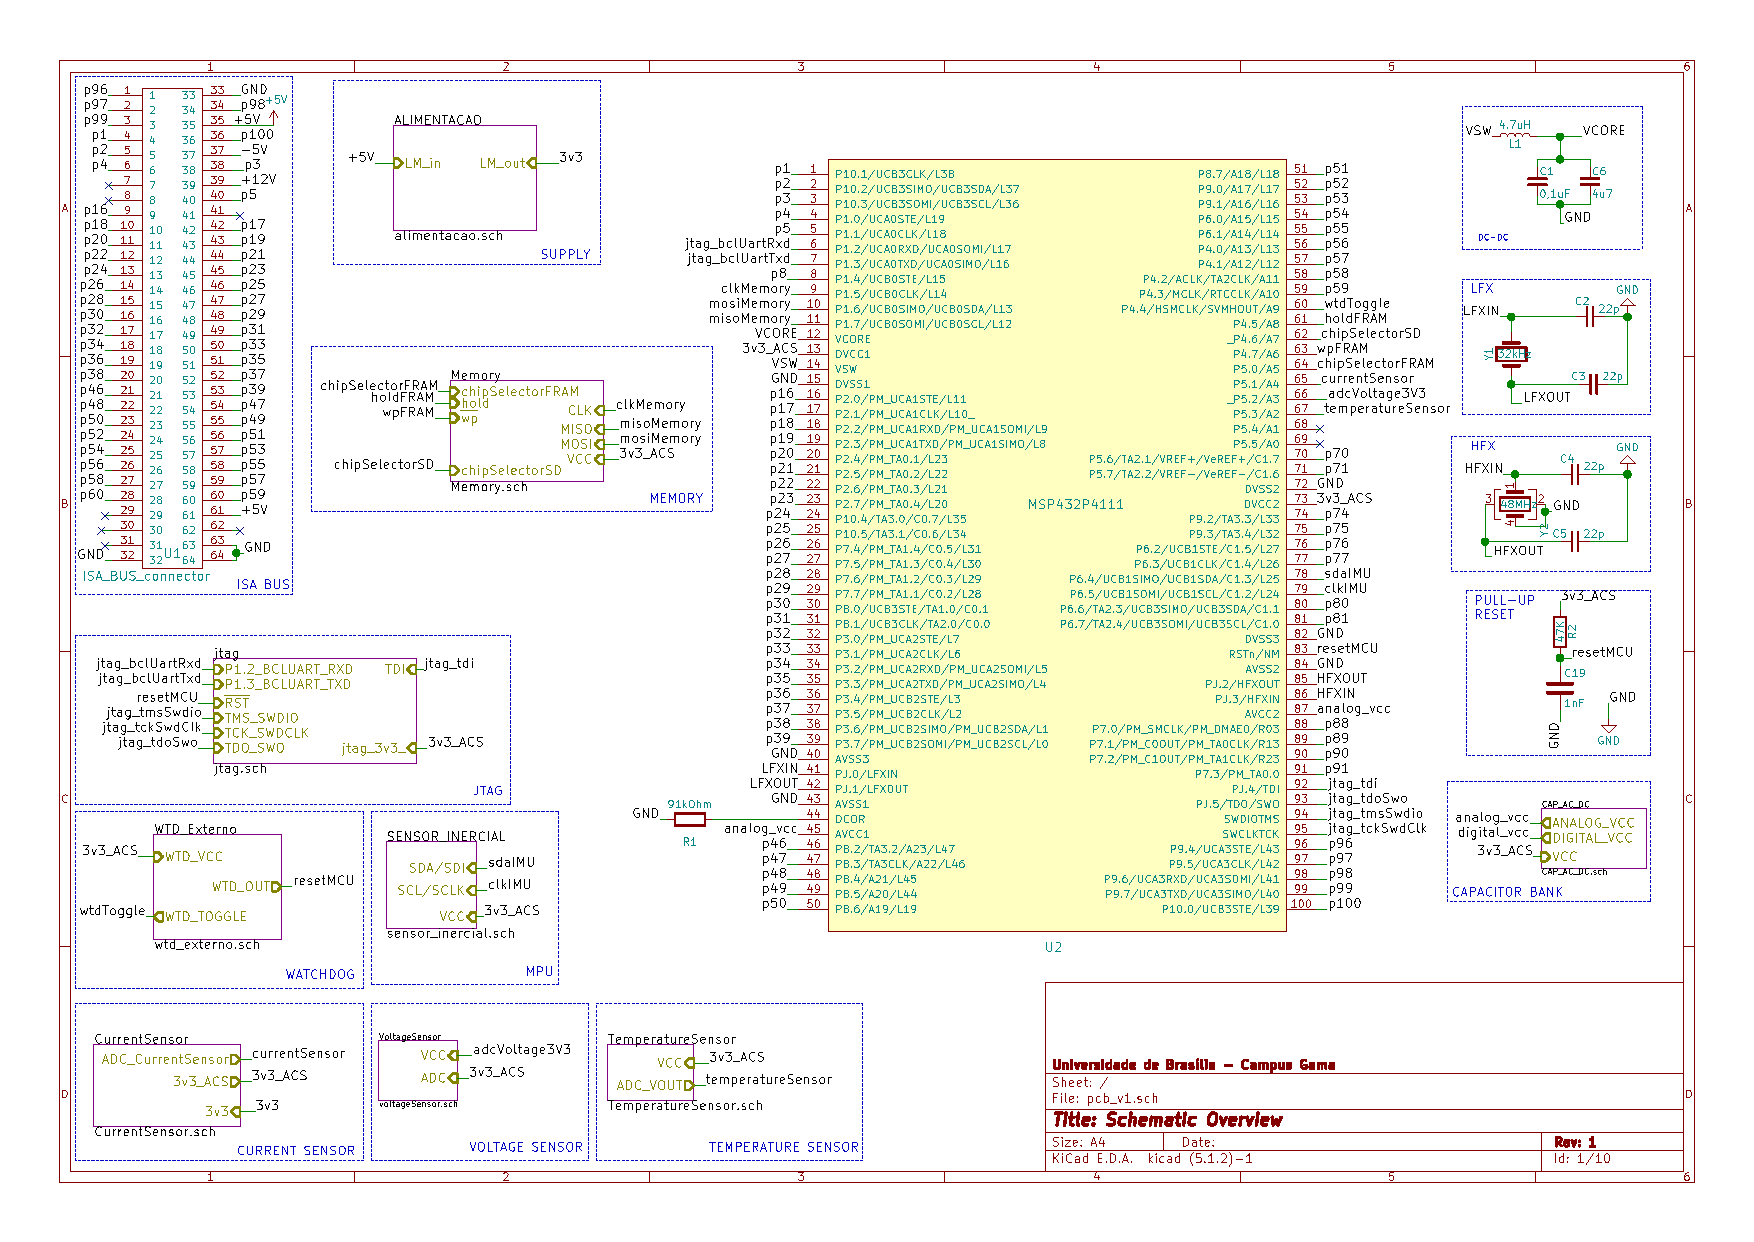
\includegraphics[page=1,width=1.1\textwidth]{pcb_v1.pdf}
	\end{tabular}
	\caption{Esquemático Eletrônico do OBC.}
	\label{fig:Test}
\end{figure}

\begin{figure}[h]
	\centering
	\begin{tabular}{@{}c@{\hspace{.5cm}}c@{}}
		\includegraphics[page=2,width=1.1\textwidth]{pcb_v1.pdf}
	\end{tabular}
	\caption{Esquemático Regulador de Tensão.}
	\label{fig:Test}
\end{figure}

\begin{figure}[h]
	\centering
	\begin{tabular}{@{}c@{\hspace{.5cm}}c@{}}
		\includegraphics[page=3,width=1.1\textwidth]{pcb_v1.pdf}
	\end{tabular}
	\caption{Esquemático Banco de Capacitores.}
	\label{fig:Test}
\end{figure}

\begin{figure}[h]
	\centering
	\begin{tabular}{@{}c@{\hspace{.5cm}}c@{}}
		\includegraphics[page=4,width=1.1\textwidth]{pcb_v1.pdf}
	\end{tabular}
	\caption{Esquemático Watchdog Externo.}
	\label{fig:Test}
\end{figure}

\begin{figure}[h]
	\centering
	\begin{tabular}{@{}c@{\hspace{.5cm}}c@{}}
		\includegraphics[page=5,width=1.1\textwidth]{pcb_v1.pdf}
	\end{tabular}
	\caption{Esquemático Sensor de Corrent.}
	\label{fig:Test}
\end{figure}

\begin{figure}[h]
	\centering
	\begin{tabular}{@{}c@{\hspace{.5cm}}c@{}}
		\includegraphics[page=6,width=1.1\textwidth]{pcb_v1.pdf}
	\end{tabular}
	\caption{Esquemático Armazenamento de Dados.}
	\label{fig:Test}
\end{figure}

\begin{figure}[h]
	\centering
	\begin{tabular}{@{}c@{\hspace{.5cm}}c@{}}
		\includegraphics[page=7,width=1.1\textwidth]{pcb_v1.pdf}
	\end{tabular}
	\caption{Esquemático Sensor Inercial.}
	\label{fig:Test}
\end{figure}

\begin{figure}[h]
	\centering
	\begin{tabular}{@{}c@{\hspace{.5cm}}c@{}}
		\includegraphics[page=8,width=1.1\textwidth]{pcb_v1.pdf}
	\end{tabular}
	\caption{Esquemático Medidor de Tensão.}
	\label{fig:Test}
\end{figure}

\begin{figure}[h]
	\centering
	\begin{tabular}{@{}c@{\hspace{.5cm}}c@{}}
		\includegraphics[page=9,width=1.1\textwidth]{pcb_v1.pdf}
	\end{tabular}
	\caption{Esquemático JTAG.}
	\label{fig:Test}
\end{figure}

\begin{figure}[h]
	\centering
	\begin{tabular}{@{}c@{\hspace{.5cm}}c@{}}
		\includegraphics[page=9,width=1.1\textwidth]{pcb_v1.pdf}
	\end{tabular}
	\caption{Esquemático Sensor de Temperatura.}
	\label{fig:Test}
\end{figure}

\begin{figure}[!h]
	\centerfloat
	\centering
	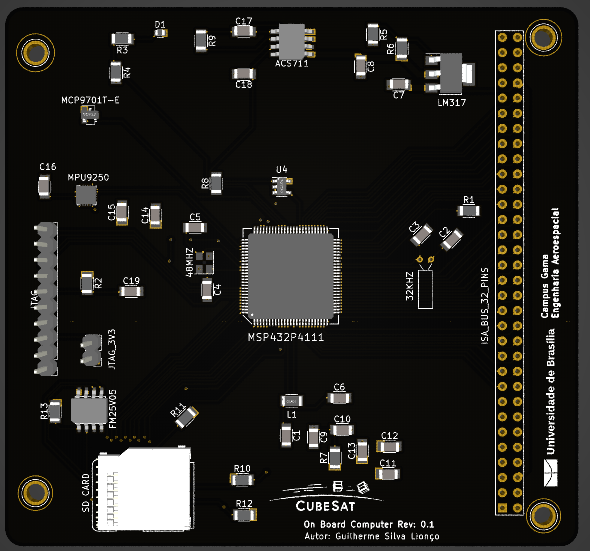
\includegraphics[keepaspectratio=true,scale=0.65]{figuras/pcbRealistic_2.PNG}
	\caption{PCB - Vista Isométrica.}
	\label{pcbRealistic_2}
\end{figure}

\begin{figure}[!h]
	\centerfloat
	\centering
	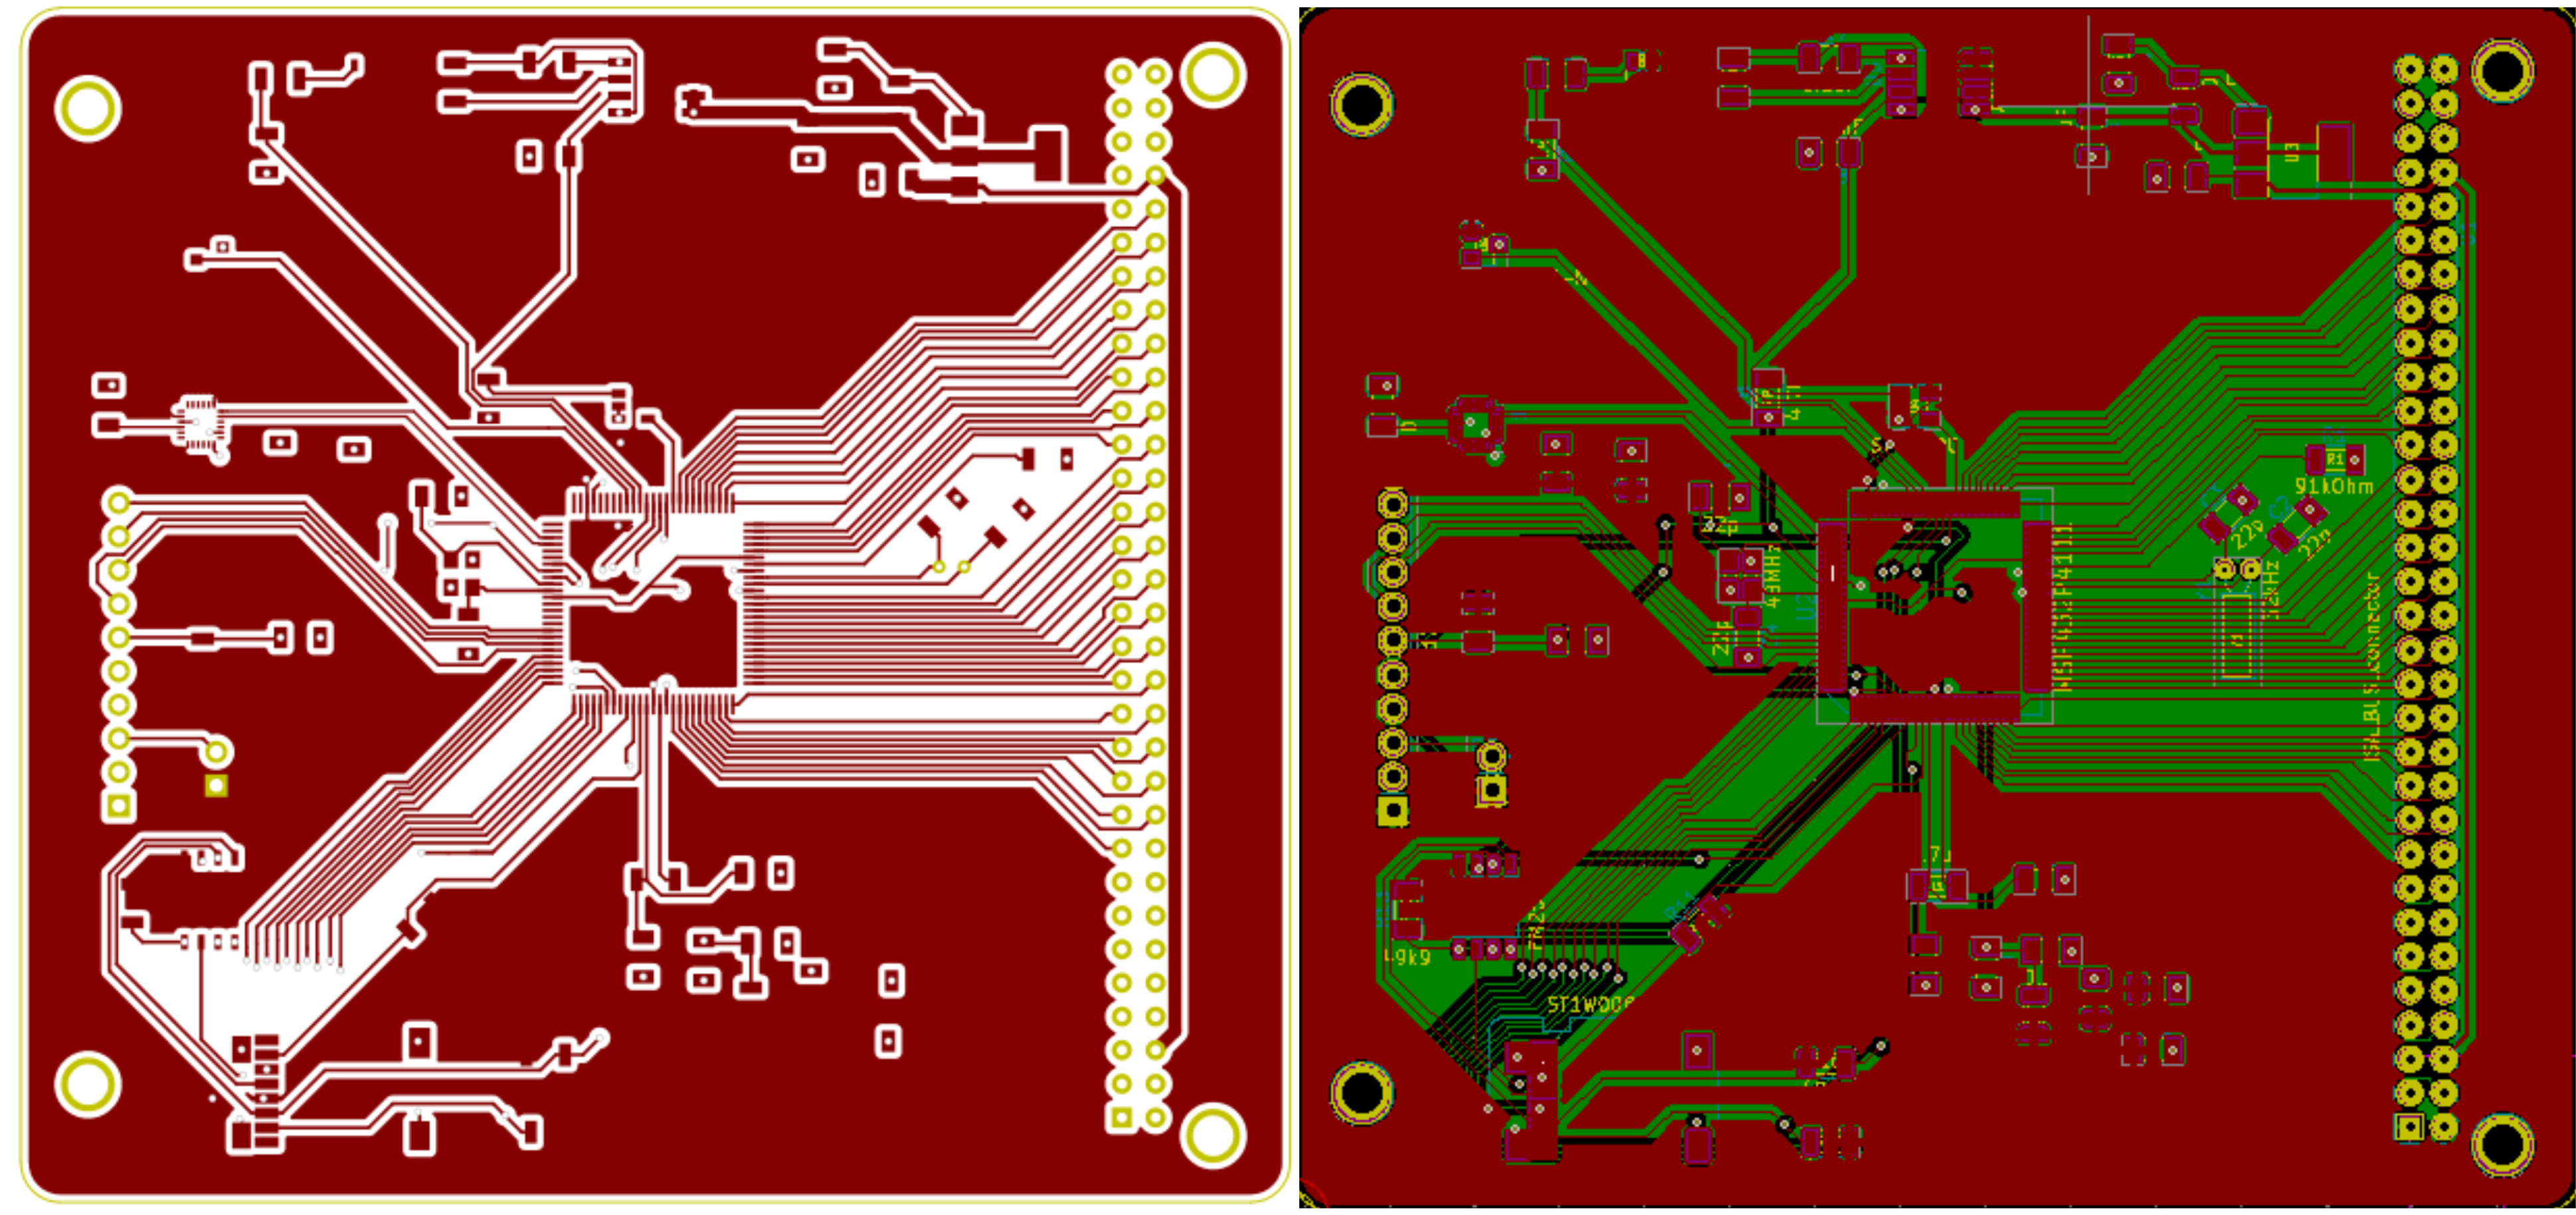
\includegraphics[keepaspectratio=true,scale=0.5]{figuras/upperLayer_.PNG}
	\caption{PCB - Plano de Cobre Superior [3V3].}
	\label{signalLayout}
\end{figure}

\begin{figure}[!h]
	\centerfloat
	\centering
	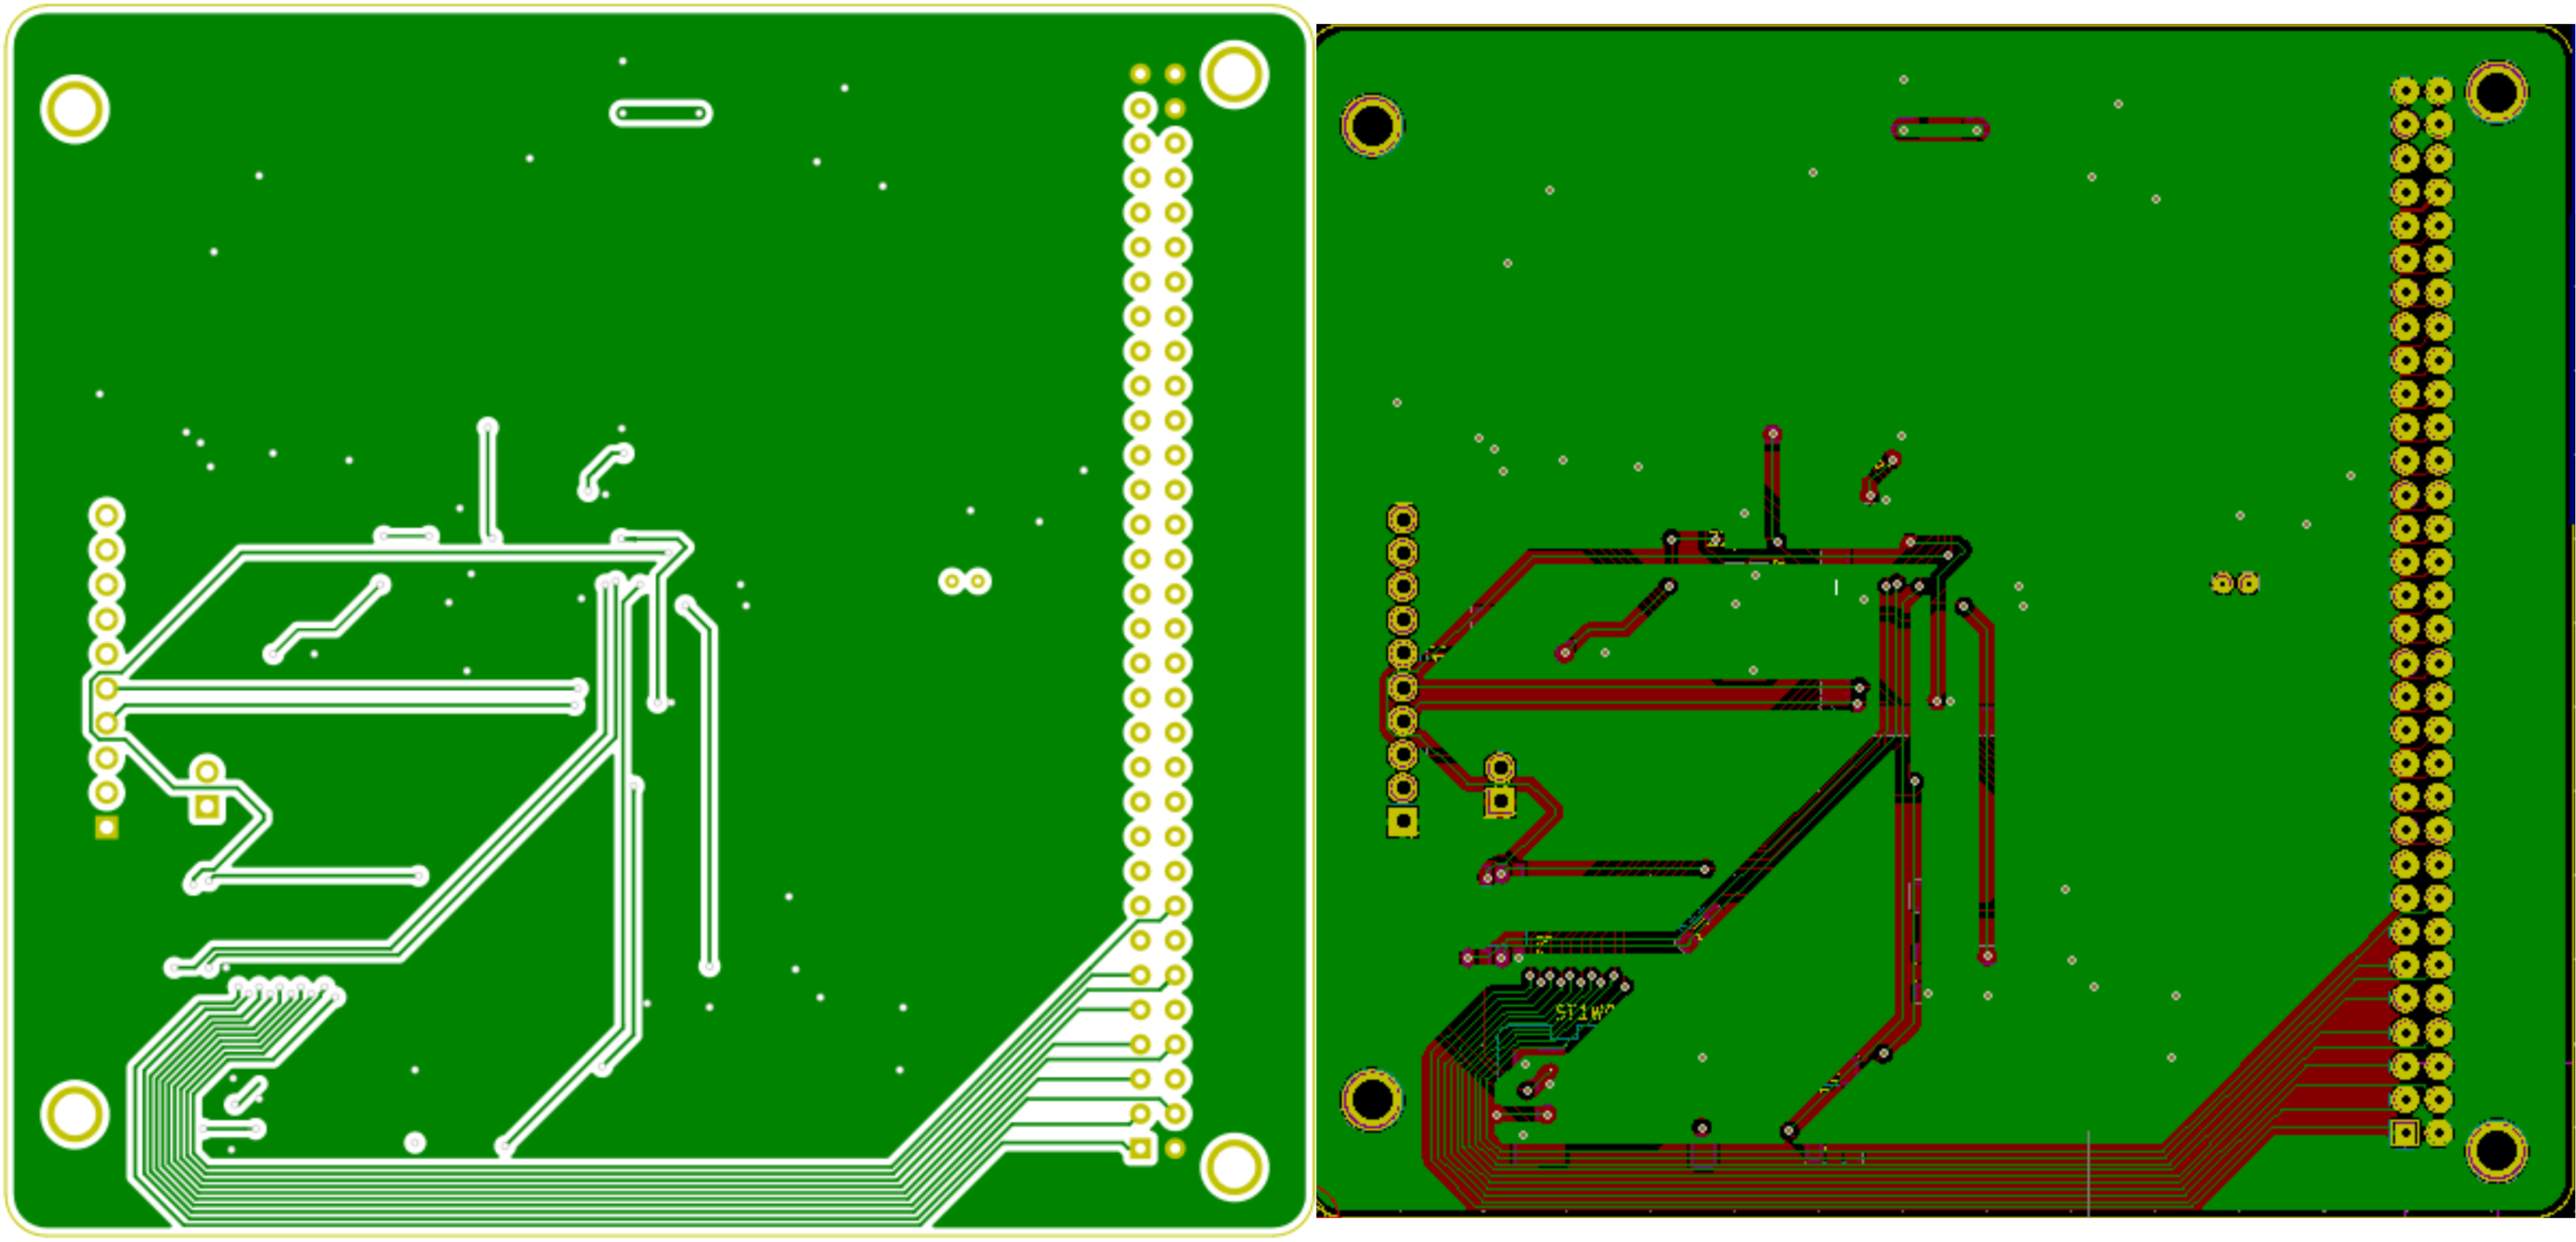
\includegraphics[keepaspectratio=true,scale=0.5]{figuras/bottomLayer_.PNG}
	\caption{PCB - Plano de Cobre Inferior [GND].}
	\label{gndSignal}
\end{figure}


\chapter{\textit{Bill of Material}}
\label{apendiceg}

\begin{figure}[h]
	\centering
	\begin{tabular}{@{}c@{\hspace{.1cm}}c@{}}
		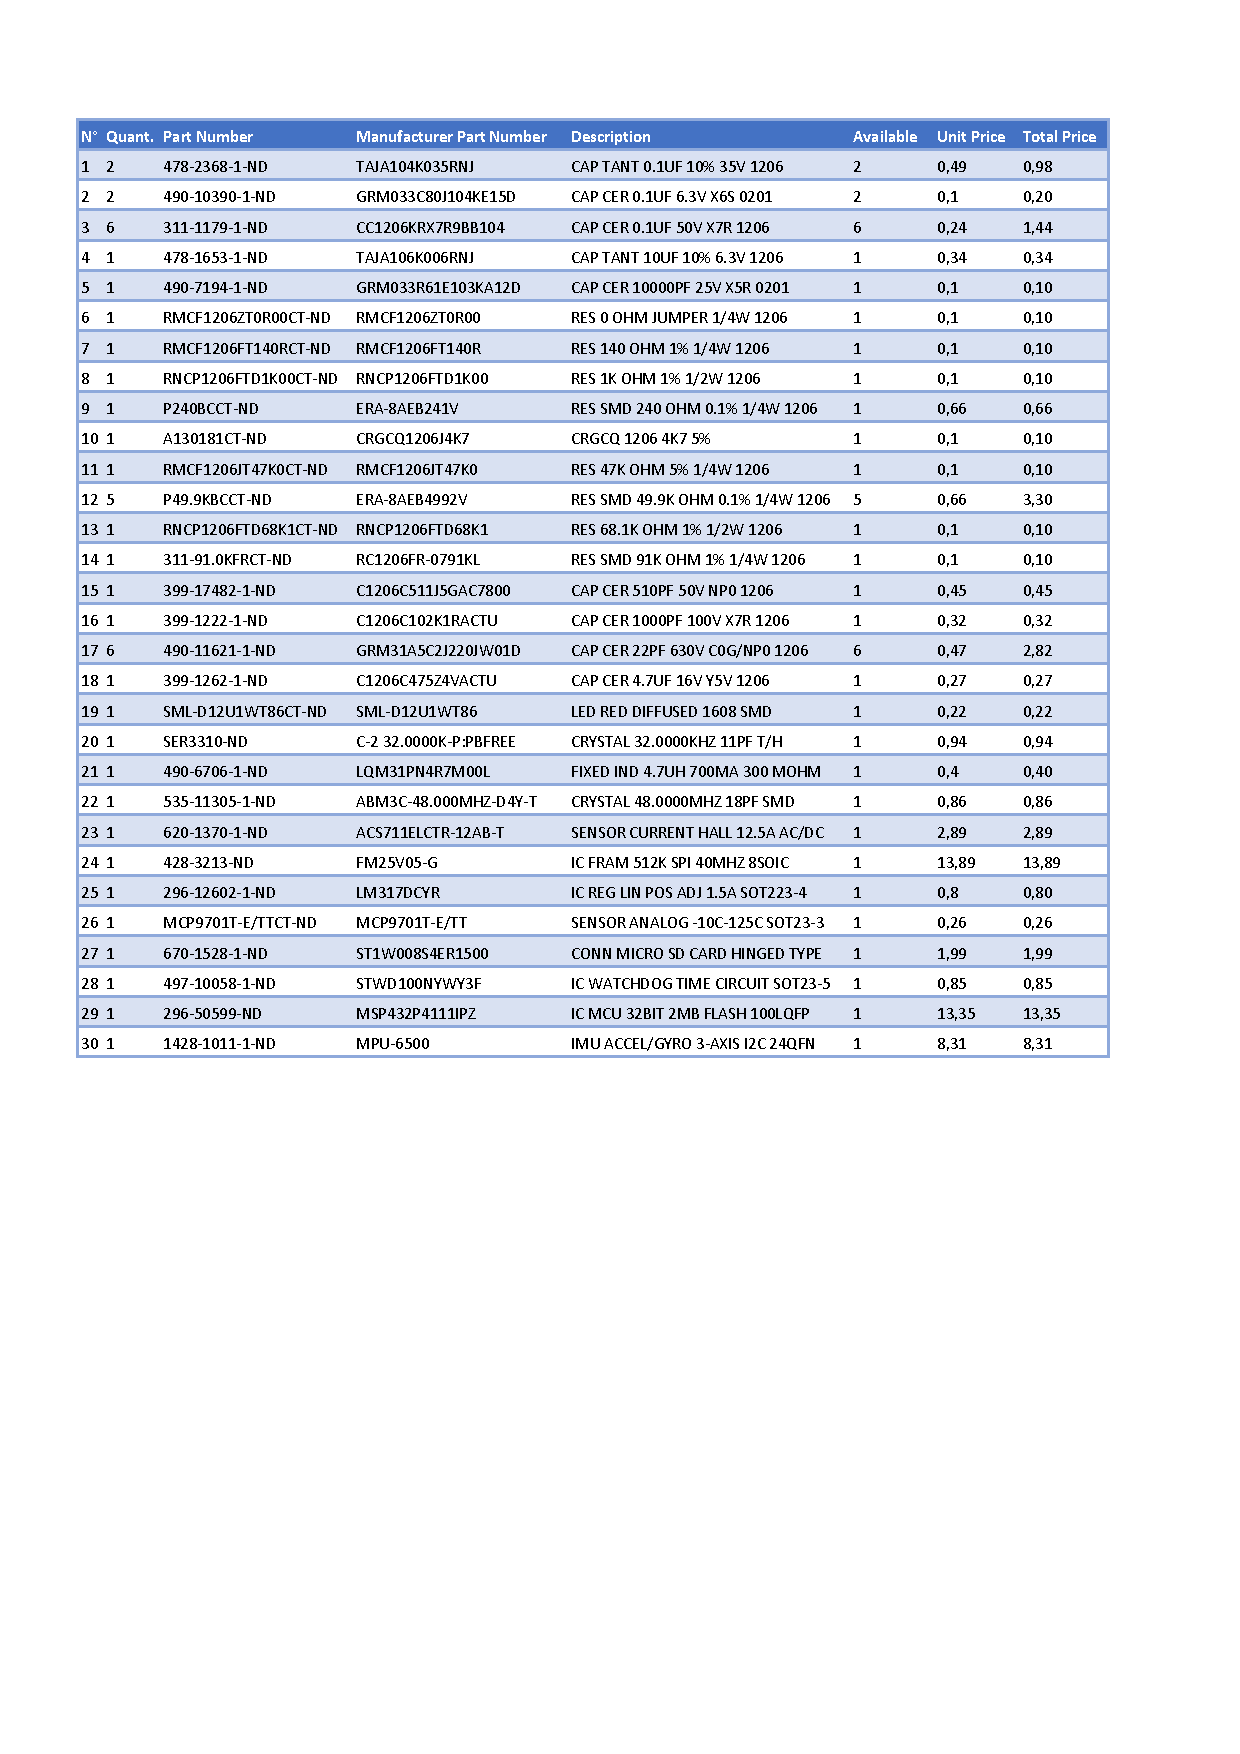
\includegraphics[page=1,width=0.920\textwidth]{figuras/bom_v1.pdf}
	\end{tabular}
	\caption{\textit{Bill of Material} do OBC}
	\label{fig:Test}
\end{figure}


\chapter{Fluxogramas da Camada de Serviço}

\label{apendicef}

Este apêndice contem os fluxogramas da Camada de Serviço do Software Embarcado.

\begin{figure}[!h]
	\centerfloat
	\centering
	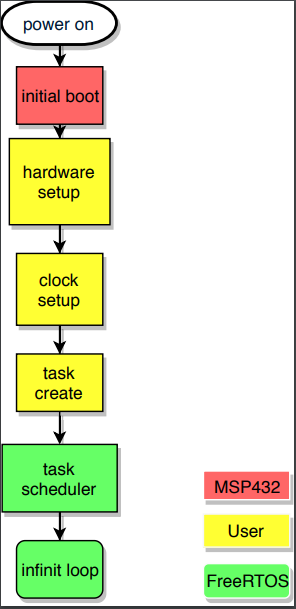
\includegraphics[keepaspectratio=true,scale=0.65]{figuras/flowChart_obc.PNG}
	\caption{Fluxograma de Inicialização.}
	\label{flowChart_obc}
\end{figure}

\begin{figure}[!h]
	\centerfloat
	\centering
	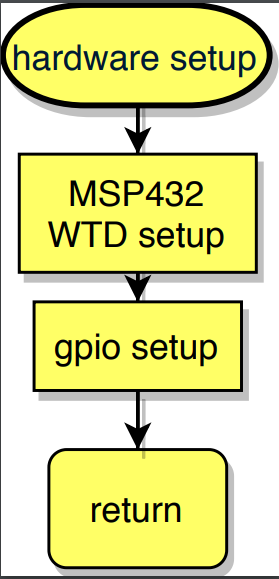
\includegraphics[keepaspectratio=true,scale=0.4]{figuras/flowChart_hardware.PNG}
	\caption{Fluxograma de Inicialização do Hardware.}
	\label{flowChart_hardware}
\end{figure}

\begin{figure}[!h]
	\centerfloat
	\centering
	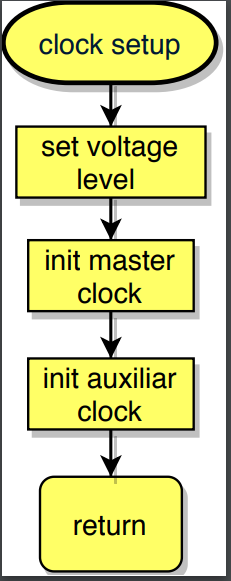
\includegraphics[keepaspectratio=true,scale=0.4]{figuras/flowChart_clockSetup.PNG}
	\caption{Fluxograma de Inicialização do Clock.}
	\label{flowChart_clockSetup}
\end{figure}

\begin{figure}[!h]
	\centerfloat
	\centering
	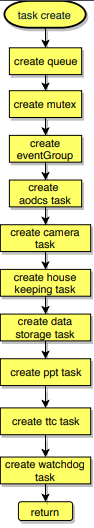
\includegraphics[keepaspectratio=true,scale=0.85]{figuras/flowChart_taskCreate.PNG}
	\caption{Fluxograma de criação das \textit{Tasks}.}
	\label{flowChart_taskCreate}
\end{figure}

\begin{figure}[!h]
	\centerfloat
	\centering
	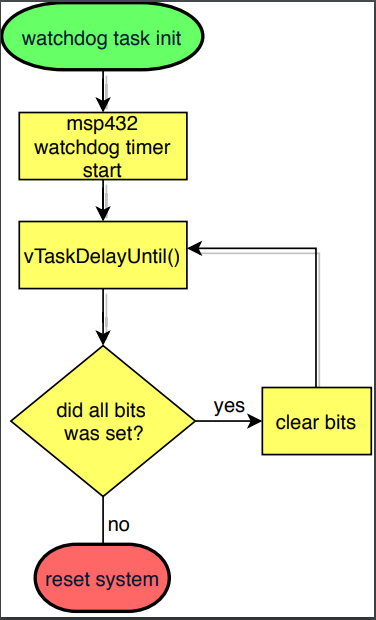
\includegraphics[keepaspectratio=true,scale=0.35]{figuras/flowChart_wdt.PNG}
	\caption{Fluxograma do \textit{Watchdog Task}.}
	\label{flowChart_wdt}
\end{figure}

\begin{figure}[!h]
	\centerfloat
	\centering
	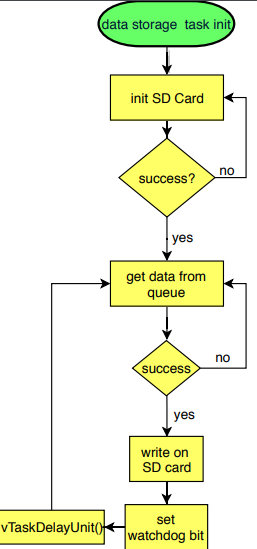
\includegraphics[keepaspectratio=true,scale=0.5]{figuras/flowChart_dataStorage.PNG}
	\caption{Fluxograma do \textit{DataStorage Task}.}
	\label{flowChart_dataStorage}
\end{figure}

\begin{figure}[!h]
	\centerfloat
	\centering
	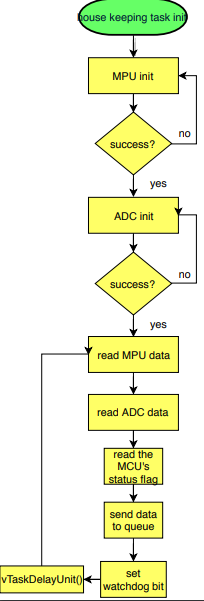
\includegraphics[keepaspectratio=true,scale=0.45]{figuras/flowChart_houseKeeping.PNG}
	\caption{Fluxograma do \textit{HouseKeeping Task}.}
	\label{flowChart_houseKeeping}
\end{figure}


\end{apendicesenv}